\subsection{Baseline}
Dense video captioning is a challenging task that involves both event localisation and event captioning. The two subtasks are typically solved in a two-stage pipeline, but there are a number of limitations to this approach. End-to-end models for dense video captioning have the potential to improve the performance of both subtasks, but they are also more complex and require a large amount of training data. 

Our initial approach is to address video captioning in a rudimentary manner. For the purpose of generating concise video descriptions, we utilise the InceptionV3 \cite{Szegedy2015RethinkingTI} model with pre-trained ImageNet weights to extract image features. We then use a transformer with multi-head attention to combine the image captions and features to obtain the final output. We proceed to extract keyframes from the video and generating captions for each frame separately using the trained transformer. Subsequently, we seek to combine the individual captions to form a coherent paragraph describing the video content. Finally, we leverage ChatGPT to understand if it could stitch the pieces together and help us gain a deeper understanding of the video context to produce a more comprehensive and insightful description as opposed to doing this with an end-to-end system.

At first, we configure the image feature extraction model. The InceptionV3 model is replicated up to its penultimate layer. This allows us to obtain only the output tensor that represented the feature vector of each input image by removing the classification layer. We re-scale all images to a size of 299 $\times$ 299 and set the batch size to 16. The vocabulary size of image captions in the Flickr8k dataset is $\approx$ 8800. We refine the captions through various preprocessing steps, including the removal of stop-words, numerals, and punctuation marks. They are then tokenised, with the out-of-vocabulary words being replaced by the \textit{<unk>} token. Markers for the beginning and end of sentence are also added. A tokeniser is then fit on the training captions and used to convert the text to sequences of integers. The resulting sequences are zero-padded and returned as a caption vector with dimensions (40000, 31). We use an 80/20 train/test split and pre-fetch the dataset in batches of size 64.
\begin{figure*}[htbp] % use the figure* environment to span both columns
  \centering
  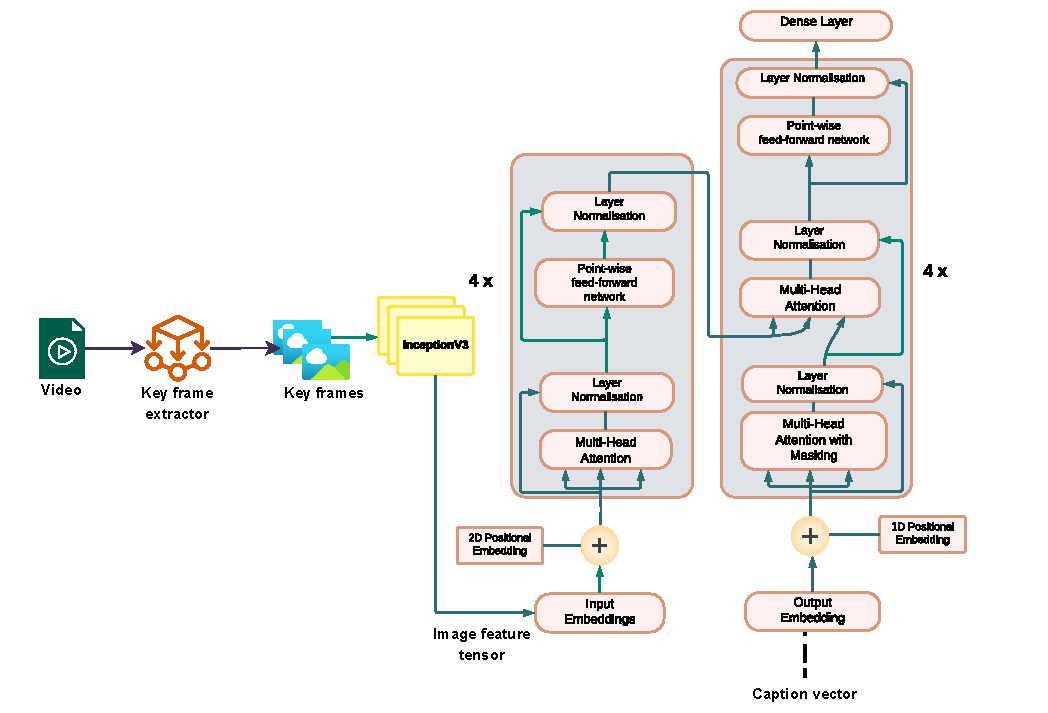
\includegraphics[scale=0.6]{images/baseline.pdf} % set the width to the full text width
  \caption{Our baseline model's architecture, which comprises a video key-frame generator, an image feature extractor, and a vanilla transformer}
  \label{fig:baseline}
\end{figure*} 
As for the transformer architecture, there are 4 encoding and decoding layers with 512 units and 8 attention heads. The size of the feed-forward layer is 2048 and the dropout ratio is set to 0.1. We calculate the attention weights by performing the scaled dot product operation, with masking added to the attention logits before applying the softmax activation function. In the forward pass of the multi-head attention module, the inputs are passed through dense layers and then split into multiple heads. The scaled dot product attention is applied to the bifurcated tensors. The resulting output is transposed, concatenated, and passed through a final fully connected layer. The point-wise feed-forward network is composed of two dense layers, where the first layer has the ReLU activation function applied to its output. In the encoder layer, the input tensor is first passed through a multi-head attention layer with masking, and then a point-wise feed-forward network. Dropout and layer normalisation are applied after each sublayer, and residual connections are added before performing normalisation. Each decoder layer consists of two multi-head attention sub-layers and one point-wise feed-forward sub-layer. The first attention sub-layer applies masked self-attention to the decoder input sequence to prevent attending to future tokens. The second attention sub-layer applies attention to the encoder output and the output of the self-attention layer. The feed-forward layer acts on the output of the second attention. The layers also contains residual connections and layer normalisation for each sub-layer. Additionally, the encoder and decoder contain embedding and positional encoding layers for the image and caption data, respectively. To prevent the decoder from attending to future tokens and to mask out padding tokens in the target sequence, look-ahead and padding masks are created. We use a custom learning rate scheduler that gradually increases the learning rate during the first 5000 steps and gradually decreases it afterwards. Moreover, we use sparse categorical cross entropy loss that effectively masks out the loss over padded values in the input sequence. The loss function returns the average loss per non-padded token in the batch. Finally, the model's parameters are optimised over 20 epochs by applying gradients using the Adam optimiser during the training process.

The implementation is done using Tensorflow with $\approx$ 35M trainable model parameters. The checkpoints are stored and retrieved during evaluation. We evaluate the trained model over images in the test set by first extracting the image features. Then, we feed these features to our transformer to generate captions one word at a time, until the end of sentence token is reached. 

The last step is to processes our video files to extract keyframes. We use OpenCV to read the frames from the video file and then divide each frame into 9 blocks to compute the color histograms. We then apply singular value decomposition to obtain projections of the feature vectors onto a lower-dimensional subspace. Finally, we group the projections and selects keyframes based on a minimum similarity threshold. The keyframes are saved as individual PNG image files which are then captioned using our transformer model. The individual captions are later connected into a paragraph and given as input to ChatGPT to enhance them. Figure \ref{fig:baseline} shows the architecture of our model.

\textbf{Motivation} Is it possible for this simple approach to yield results that are comparable to those of end-to-end models? If not on their own, how do the descriptions generated by ChatGPT compare to the results produced by other models?

\subsection{PDVC}
PDVC \cite{le2021pdvc} is an end-to-end dense framework that uses parallel decoding and directly feeds the intermediate representation into a captioning head, bypassing the two-stage “\textit{localise-then-describe}” scheme. This approach aims to leverage inter-task association at the feature level, allowing the intermediate feature vectors to be matched with target events on a one-to-one basis, making the feature representations more distinct to identify a particular event. It is built upon the "\textit{localise-select-describe}" pipeline, which was first introduced by SDVC, an RNN-based model \cite{Mun2019StreamlinedDV}, to address issues such as caption redundancy, incoherence and the generation of a large volume of proposal-caption pairs. It is scaled to be used in an end-to-end solution that eliminates the need for multi-step training or a recurrent architecture that is often limited in its ability to handle videos with a large number of events.  It is trained on the ActivityNet and YouCook2 datasets.

\textbf{Deformable Transformer} Is a novel architecture whose encoder-decoder structure allows the model to capture the inter-frame, inter-event, and event-frame interactions using its multi-head attention mechanism and produces a set of event query features, which are then used to predict the boundaries and captions simultaneously. This module allows the model to attend to a sparse set of sampling points around reference points and hence mitigates the slow convergence problem of the self-attention mechanism in the Transformer model \cite{Vaswani2017AttentionIA}. It can be formalised as 
\begin{equation}
\mathrm{MSDAtt}(qj, pj, X) = \sum_{l=1}^L \sum_{k=1}^K A_{jlk} W_l X_{pjlk} \phi_l(pj) + \Delta_{pjlk}
\end{equation}
where: $A_{jlk}$ = attention weight between query element $j$ and key element $k$ at scale $l$,
$W_l$ = projection matrix for key elements,
$X_{pjlk}$ = value element at position $(pj,lk)$,
$\phi_l(pj)$ = normalized reference point at scale $l$,
$\Delta_{pjlk}$ = sampling offset at scale $l$. The input is a set of multi-scale feature maps ${X}=\{{x}^l\}_{l=1}^{L}$, a query element $q_j$, and a normalised reference point $\phi_l(p_j) \in [0,1]^2$ while the output is a context vector that contains the weighted sum of $K \times L$ sampling points taken from the feature maps across $L$ scales. K and L are set to 4 while the number of attention heads is 8. The attention dimension is 256 and the size of the feed-forward network is 1024.

\textbf{Feature\,Extraction} We use the R2Plus1D TSP on ActivityNet MaxGVF Backbone architecture \cite{r2plus1d} for determining the frame-level features. The model uses a ResNet-style 3D convolutional neural network (CNN) as the backbone, with temporal segment pooling (TSP) and maximum global video feature (GVF) pooling. The CNN has 34 layers and uses 1x1, 3x3, and 1x1 convolutions in the spatial and temporal dimensions. The TSP operation divides each video into several equal-length segments and pools features within each segment to produce a fixed-length representation of the video. The GVF operation pools features from all segments to produce a single representation of the video. The model is trained using binary cross-entropy loss, with a learning rate of 0.0001 for the backbone and 0.002 for the fully connected layer. The final layer of the model is a fully connected layer with a sigmoid activation function that outputs a probability of the input video belonging to a given activity class. This layer is removed and the pre-trained weights from the remaining layers are loaded into the PDVC model. The feature maps are re-scaled and given as input to the transformer to extract inter-frame relationships.

\textbf{Decoding} Makes use of three types of attention heads. The first of these is the localisation head which utilises a multi-layer perceptron to determine the beginning and end points of an event segment, as well as its confidence score. This is achieved by using the ground-truth segment with a reference center point. The output is the representation of form $ \{t_{s_j}, t_{e_j}, c_{loc_j}\}_{j=1}^N $ for the detected event. While the lightweight captioning head uses an LSTM to predict the next word given an event-level query, the standard captioning head enforces the relationships between words and frames using the deformable soft attention (DSA) module by spanning attention weights over a small area around the reference point. These context features along with the event query features and previous words are concatenated and given to the LSTM and the probability for the next word is obtained by an FC layer with softmax activation. The final component is the event counter that helps find an even balance between tight and sparse sampling of events by max-pooling an event query and subsequently passing it through an FC layer with softmax activation to predict a probability for the possible number of events $r_{len}$ from a global view. During evaluation, the top $N_{set}$ events with accurate boundaries and captions are selected. The confidence score for each event query is calculated using the average of the logarithm of the word probabilities for all the words in the generated caption along with the modulation factors $\gamma$ and $\mu$, to reduce exaggerated confidence for shorter sentences. Finally, the prediction is calculated as the weighted sum of the gIOU, focal and cross-entropy caption losses.

\textbf{Motivation} Can the R2Plus1D TSP backbone architecture provide good captions for our test videos? How closely do the top-\textit{k} descriptions for each frame match the content of the video? Can ChatGPT improve the quality of these descriptions?

\subsection{MART}
MART \cite{liu2020mobile} is a model for video captioning that extends the basic transformer architecture by incorporating a memory-augmented recurrence component. This approach overcomes the limitation of the vanilla transformer to retain extensive sentence and video histories, leading to improved performance in video captioning.
The goal is to generate a coherent video paragraph that describes the content of a video $V$, which consists of multiple event segments $[e_1,e_2,\dots,e_T]$ with sentences $[s_1, s_2, \dots, s_T]$ that describe each event $e_t$ in order.

The video and text embeddings are concatenated $H_0 = [H_{0, \text{video}}; H_{0, \text{text}}]$ and provided as input to MART which has an integrated encoder-decoder architecture. Token type embedding vectors are utilized to distinguish between the embeddings of text and video. The external memory module concatenates the information from its memory states $M^l_{t-1}$ and the intermediate hidden states of the encoder $H^l_{t}$ to update the memory in the current iteration to $M^l_{t}$. Meanwhile, the hidden state representation $H^l_{t}$ is augmented using $M^l_{t-1}$ and passed through a multi-head attention layer before being encoded by the normalisation and residual connection layers inside the transformer block. The model is trained on the ActivityNet and YouCook2 datasets.

\textbf{Motivation}
Before testing MART on our own videos, we train it on ActivityNet captions using a smaller batch size and a reduced number of training epochs. Our aim is to assess whether this approach still produces satisfactory results and if ChatGPT can enhance the quality of the output captions.

\subsection{DenseCap}
DenseCap \cite{johnson2016densecap} is a comprehensive end-to-end model consisting of an encoder, a proposal decoder, and a captioning decoder. It encodes the features of video frames with an encoder, and uses a proposal decoder to determine the start and end timestamps for different proposals by anchoring them. A captioning decoder then decodes the representation specific to the proposal with the help of a masking network. The proposal and captioning decoder are trained consistently using the mask, which allows the proposal module to adjust its prediction based on the quality of the generated caption. It is trained on the ActivityNet and YouCook2 datasets.

\textbf{Video\,Encoder} Encodes each frame of the video $X=\{x_1, \dots, x_T\}$ as a continuous representation $F_0=\{f_{0,1},...,f_{0,T}\}$ and feeds it through 2 encoding layers. Each layer learns a representation of the form 
\begin{equation}
 V(F_l) = \Psi(PF(\Gamma(F_l)),\Gamma(F_l)) 
\end{equation}
where $F_l$ is the input it receives from the previous layer. $\Gamma$ is the representation the self-attention mechanism with 8 attention heads and an attention space of dimension 1024. Each output time-step captures the complete context information by considering a weighted sum of all previous time steps for each query $f_l^t$. The network also includes a 2-layer feed-forward network $PF$ with ReLU activation applied on the first linear layer. Additionally, residual connections and layer normalisation $\Psi$ are applied to both the attention and feed-forward segments. A dropout ratio of 0.2 is used for the attention weights and the residual blocks. The dimension of the feed-forward layer is 2048.

\textbf{Proposal Decoder} The anchor offset mechanism is adapted from ProcNets \cite{Zhou2017TowardsAL}. The event proposal boundaries $(\mathrm{S_p}, \mathrm{E_p})$ are computed using the center and length offsets $\theta_c$ and $\theta_l$, as well as the anchor length $l_a$ and center $c_a$ parameters, respectively. The confidence for each event proposal score is $\mathrm{P_e} \in [0,1]$. The decoder receives the output from the video encoder as its input. It is made up of 3 1D convolutional and batch normalisation layers. ReLU non-linearity is applied at the hidden layer. The kernel size varies from 1 to 251 while the stride factor is set to 50. The stride size varies as a function of the kernel size and stride factor and acts as a preventive measure to avoid long event sequences. 

\textbf{Captioning Decoder} The captioning decoder, as stated earlier makes use of the Masked Transformer to generate natural sentence. For a given word vector $Y^l_{\leq t}$, the 2-layered decoder leverages $\Omega$ to compute the self-attention. It then calculates the element-wise product $\odot$ between the masking function $f_M: \mathbb{R}^{2} \rightarrow [0,1]^T$ over the proposal boundaries and the visual representations $\{F^1 \dots F^l\}$ from the video encoder. The function takes non-zero values near the proposal boundaries and approaches zero elsewhere. More specifically, this masking function prompts the encoder (read video encoder) block of the transformer to regenerate the visual features so as to contain only the information relevant to the current proposal. The masked visual representation from the feed-forward layer of the encoder are then combined with the output of the self-attention layer using $\Psi$ to generate a cross-modal or multi-attention representation, which is then used to predict the probability distribution over the next word in the caption using a linear layer with softmax activation. The final result is thus the probabilities for $w_{t+1}$ which is computed over the product of the word-embedding matrix $W^v$, of vocabulary size $v$ and the decoder output $y_{t+1}$. The dropout ratio is set to 0.2 while the transformer dimension is retained at 1024 units.

\textbf{Differential Proposal Mask} Is the fully differentiable masking function $f_m$ that is computed as a function of 
a parameterised MLP and the logistic sigmoid fuction. This function is especially useful for building the gated mask $f_{GM}$ which is a complementary sum of the output from the proposal decoder and $f_m$ in cases where the confidence score from the proposal decoder is low.

\textbf{Motivation}
We use the pre-trained model's weights on ActivityNet to caption our videos. However, we acknowledge that this approach can lead to repetitive information, especially in long videos where the number of captions can become excessive. Therefore, our goal is to investigate whether ChatGPT can alleviate this issue for us.

\subsection{SwinBERT}
SwinBERT \cite{lin2022swinbert} is a cutting-edge video captioning model that adopts a transformer-based architecture to generate natural language descriptions from video frame patches used as direct inputs. It encodes spatial-temporal representations in a novel way, eliminating the need for multiple computational intensive 2D appearance/3D motion feature extractors which operate on steadily sampled frame rates, as in traditional video captioning methods. Furthermore, this model can handle varying video input lengths with ease. This approach is better than the mainstream sparse sampling method that are commonly used in video-and-language understanding tasks. It is trained on the VATEX, MSRVTT, MSVD, TVC and YouCook2 datasets. It is adept at sampling denser video frames and can thus be relied upon to generate high-quality video captions. The architectural construct is described as follows.

\textbf{Video Swin Transformer} The VidSwin \cite{Liu2021VideoST} model is employed to address the hazard of stacking numerous frames to achieve long-term temporal modeling, which is seminal for effective video understanding. By using the visual encoder with pre-trained Kinetics-600 weights, we can capitalise on its ability to leverage the spatio-temporal locality present in videos, resulting in a balanced trade-off between speed and accuracy. The video frames in their raw form have dimensions of $T \times H \times W \times 3$, where $T$ represents the number of frames and each frame contains $H \times W \times 3$ pixels. The grid features of these frames of dimensions $\frac{T}{2} \times \frac{H}{32} \times \frac{W}{32} \times 8C$, are extracted from the $4^{th}$ and final stage of the Swin transfomer block and dissected 8-ways along the channel dimension $C$, before being sent into the multi-model encoder for caption generation. $T$ is set to 128.

\textbf{Multi-Modal Transformer Encoder} Observes inputs from both caption descriptions and video tokens and performs sequence-to-sequence generation to produce a coherent sentence. The use of a causal self-attention mask allows the encoder to generate output tokens in a uni-directional sense, with each output caption token riveting its focus to its own ground-truth input counterpart. The text tokens are able to access all video tokens, providing additional information about the scene encapsulated by the frames. This allows them to better understand the context of the video and generate more accurate and descriptive captions. Moreover, a trainable sparse attention mask using the sigmoid activation function is employed to regularise the encoder and mitigate issues arising from redundant information in densely sampled consecutive long-input video frames. The dimensions of the attention mask are $(N + M) \times (N + M)$ where $N = 50$ is the length of the textual tokens and $M$ is the size of the single-channel grid features obtained from \textit{VidSwin}. The sparsity constraint \begin{equation}
\mathrm{L_{SPARSE}} = \lambda \cdot M \sum_{i=1}^{M} \sum_{j=1}^{|V_{i,j}|}
\end{equation}
with the regularisation term $\lambda$ and activation values $V_{i,j}$ is used to impose the learnable attention mask $V$ of size $M \times M$ over the video tokens. Over time, the model discovers the most meaningfully rich and high-impact video tokens and forbids connections to inactive tokens with weak correlations.

Moreover, to facilitate the learning of representations that capture the relationship between text and video tokens, a masked language model is used. This involves randomly covering some of the input text tokens using the special token $\mathrm{[MASK]}$, and predicting the most probable value for them based on the surrounding text and video tokens. For generating captions during testing, the model produces one token at a time, taking the previously generated tokens as inputs to the encoder and terminates when the $\langle${eos}$\rangle$ tag is encountered. An MLP is applied to the video tokens to match the sizes of their embeddings with those of the text tokens. The weights are optimised using AdamW \cite{Loshchilov2017DecoupledWD}.

\textbf{Motivation}
Our motivation stems from the following thought – for videos that are extremely long, captioning models may fail due to the need to encode long-term dependencies, which requires structures like memory banks or knowledge graphs to be incorporated \cite{Pan2020SpatioTemporalGF}. Instead of captioning an entire video, what if we are to break them down into \textit{n} partitions, generating individual captions for each of these, and then combining them into a comprehensive description using a large language model like GPT-3? In other words, can ChatGPT effectively decipher the meaning of the video by analyzing the individual captions of each clip despite using such a segmented approach? We partition our test videos into 10-second clips to evaluate our hypothesis.

 VATEX is a vast multilingual video description dataset comprising more than 41,250 videos and 825,000 captions in English and Chinese, including explanations of 600 human activities. Despite SwinBERT not being trained on the ActivityNet dataset, we deem VATEX to be a fitting substitute due to its abundant clip-sentence pairs, extensive lexical content, and similarity to ActivityNet and hence leverage its checkpoints to test our results.